\section{AN\'ALISIS DE UNA OBRA DODECAF\'ONICA: OP. 25}\label{ch:suite}
	\subsection{Series de la Suite op. 25}
		Lo primero que har\'a un compositor dodecaf\'onico antes de empezar a componer ser\'a escoger su serie original. Su elecci\'on nunca es una simple cuesti\'on de azar; al contrario, ya que las singularidades de la serie dar\'an un car\'acter especial a toda la obra. Por ejemplo, el compositor puede escoger una serie con simetr\'ias, y as\'i tendr\'a series repetidas entre su espectro serial. Tambi\'en puede tener simetr\'ias internas solo en un fragmento de tres o cuatro notas, y de este modo podr\'a el compositor oscilar entre varias series del espectro que se parezcan entre s\'i.\footnote{Para un estudio m\'as completo de las relaciones de similitud entre series se recomienda \emph{On the Similarity of Twelve-Tone Rows}, de Tuukka Ilom\"aki. \cite{ilomaki}}
		
		En la Suite para Piano Op. 25, Schoenberg escoge su serie $\sigma$ para resaltar el intervalo de tritono (6 semitonos). A continuaci\'on se observan en negrita los intervalos entre las notas de esta serie, en unidad de semitono:
		
		{$\left(\begin{array}{*{24}c}
			0&&1&&2&&3&&4&&5&&6&&7&&8&&9&&10&&11&\\
			4&\mathbf{1}&5&\mathbf{2}&7&\mathbf{6}&1&\mathbf{5}&6&\mathbf{9}&3&\mathbf{5}&8&\mathbf{6}&2&\mathbf{9}&11&\mathbf{1}&0&\mathbf{9}&9&\mathbf{1}&10&\mathbf{6}\end{array}\right)$}
				
		Presenta repeticiones triples de los intervalos de tritono (6), de sexta mayor (9) y de segunda menor o semitono (1): los intervalos m\'as disonantes; una repetici\'on doble de cuarta justa (5), y un intervalo de segunda mayor (2); adem\'as de una consecuci\'on de intervalos repetida: 9 -- 1 -- 9 -- 1. Como se forma el intervalo de tritono al enlazar la serie original con una serie que empiece por la misma nota, se tiene en cuenta el intervalo de tritono (6) al final. En el dodecafonismo se evitan deliberadamente los intervalos de tercera mayor (4), ya que estos son la base de la eludida armon\'ia tonal. \label{serie25}
		
		El intervalo de tritono tiene la particularidad de no modificarse en la inversi\'on y transportaci\'on k = 6, por lo que estos intervalos aparecen en los lugares originales, mientras que en los procedimientos de retrogradaci\'on y retrogradaci\'on inversa ocupan sus lugares en retr\'ogrado. En particular, Schoenberg utiliza entre los seis movimientos de la Suite solamente las ocho series de todo el espectro serial que cumplen estos requisitos: T$^0$, T$^6$, I, IT$^6$, R, RT$^6$, RI y RIT$^6$, que podemos observar %en el Anexo \ref{app:series}, p\'agina \pageref{app:series}.
		a continuaci\'on:
		
		\chapter{Series de la Suite Op. 25}
	\label{app:series}
	
	\newpage
	$$\text{T}^0=\left(\begin{matrix}0&1&2&3&4&5&6&7&8&9&10&11\\4&5&7&1&6&3&8&2&11&0&9&10\\\end{matrix}\right)$$
	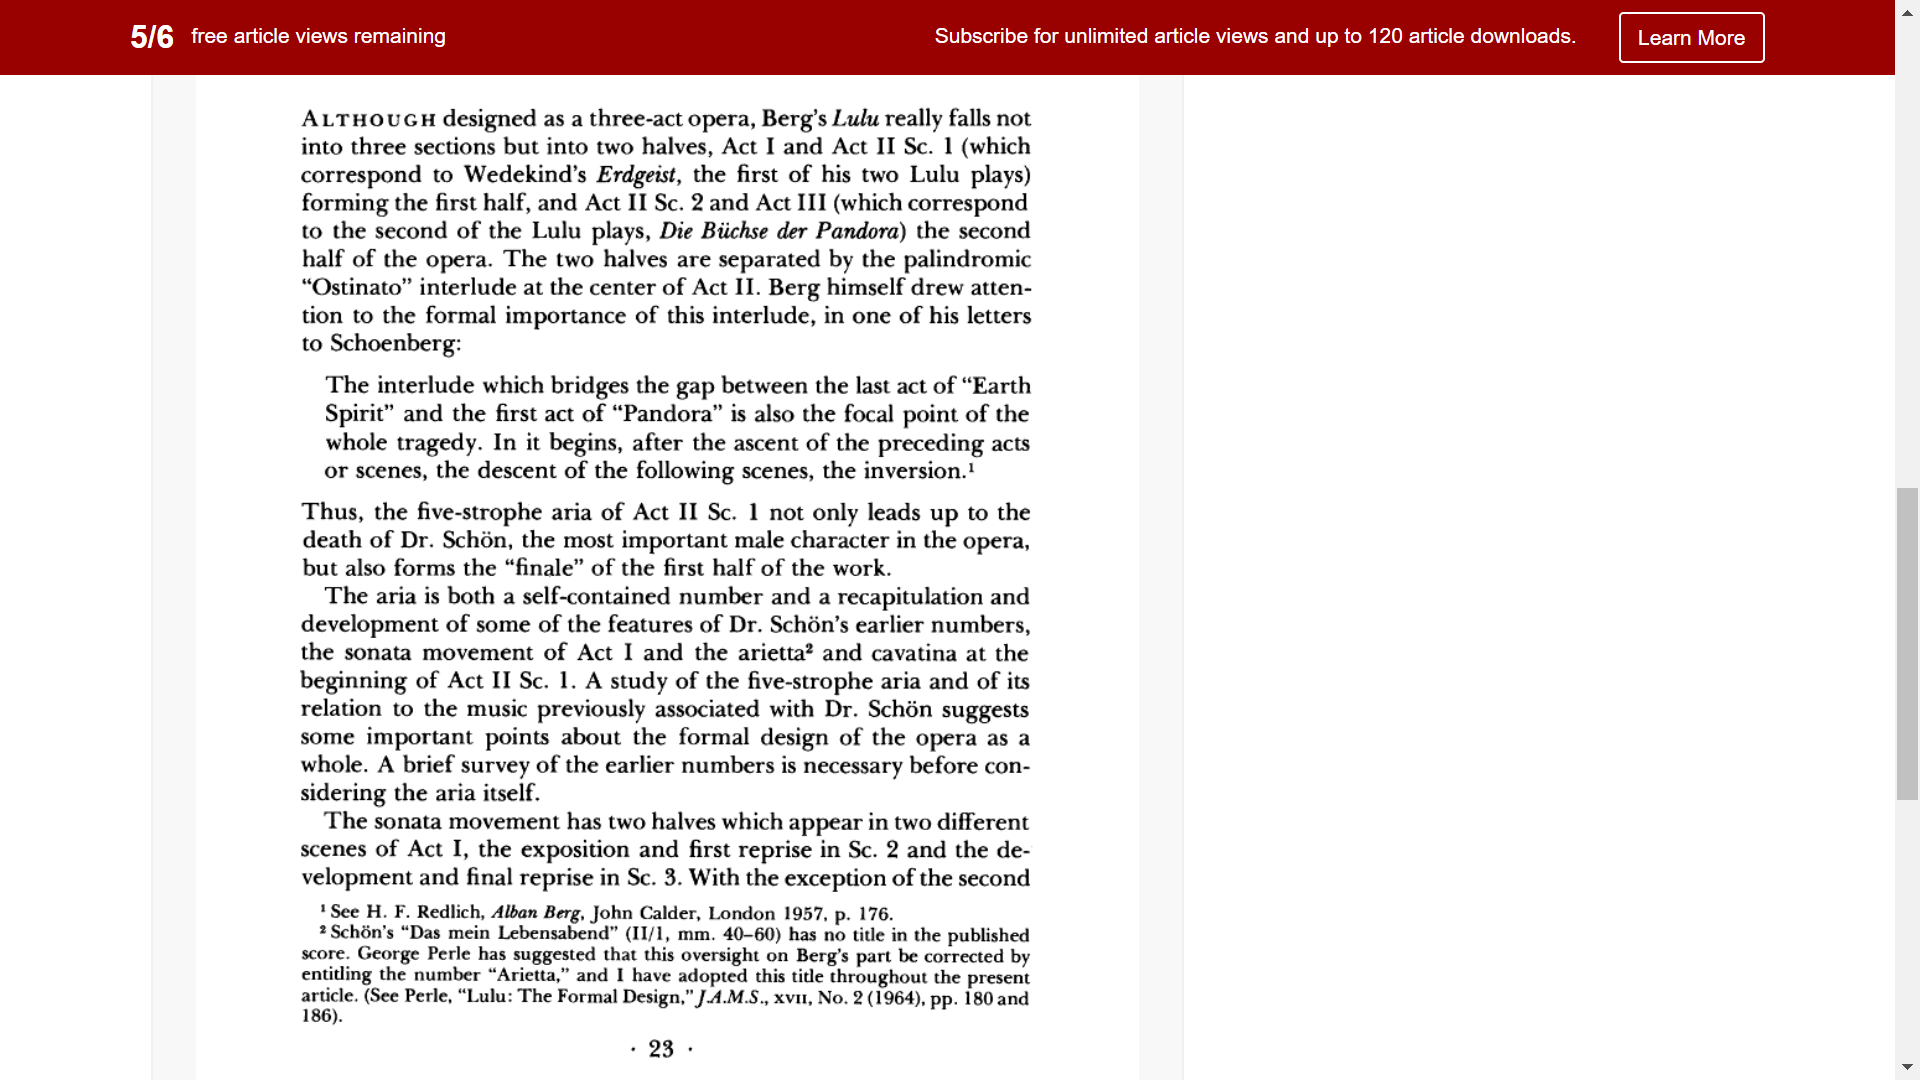
\includegraphics[width=\textwidth]{1.png}
	\bigskip\bigskip
	$$\text{T}^6=\left(\begin{matrix}0&1&2&3&4&5&6&7&8&9&10&11\\10&11&1&7&0&9&2&8&5&6&3&4\\\end{matrix}\right)$$
	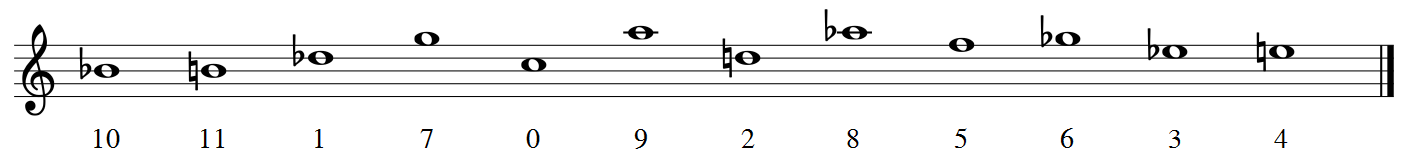
\includegraphics[width=\textwidth]{2.png}
	\bigskip\bigskip
	$$\text{IT}^0=\left(\begin{matrix}0&1&2&3&4&5&6&7&8&9&10&11\\4&3&1&7&2&5&0&6&9&8&11&10\\\end{matrix}\right)$$
	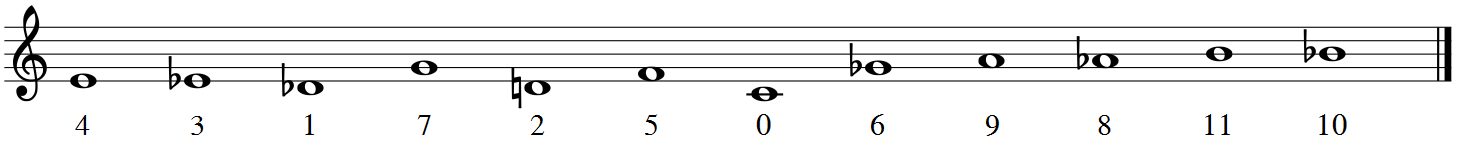
\includegraphics[width=\textwidth]{4.png}
	\bigskip\bigskip
	$$\text{IT}^6=\left(\begin{matrix}0&1&2&3&4&5&6&7&8&9&10&11\\10&9&7&1&8&11&6&0&3&2&5&4\\\end{matrix}\right)$$
	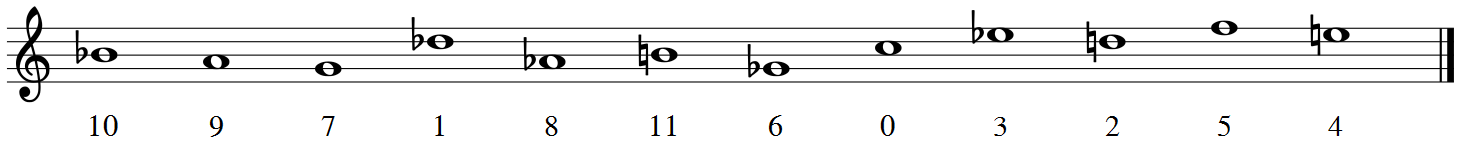
\includegraphics[width=\textwidth]{6.png}
	\newpage
	$$\text{RT}^0=\left(\begin{matrix}0&1&2&3&4&5&6&7&8&9&10&11\\10&9&0&11&2&8&3&6&1&7&5&4\\\end{matrix}\right)$$
	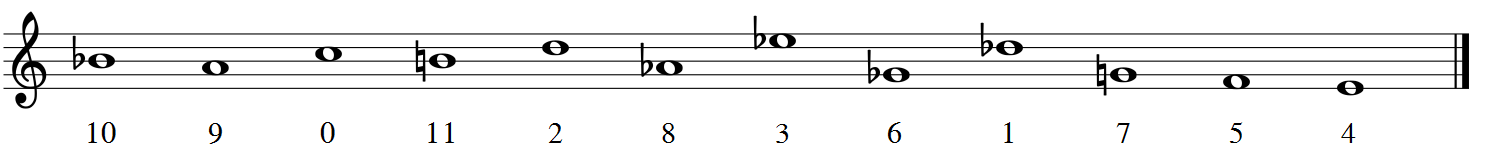
\includegraphics[width=\textwidth]{3.png}
	\bigskip\bigskip
	$$\text{RT}^6=\left(\begin{matrix}0&1&2&3&4&5&6&7&8&9&10&11\\4&3&6&5&8&2&9&0&7&1&11&10\\\end{matrix}\right)$$
	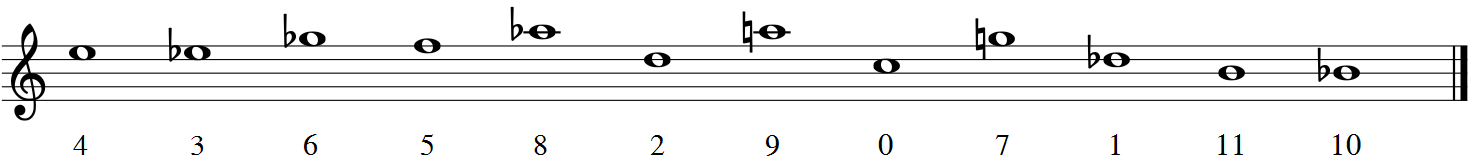
\includegraphics[width=\textwidth]{7.png}
	\bigskip\bigskip
	$$\text{IRT}^0=\left(\begin{matrix}0&1&2&3&4&5&6&7&8&9&10&11\\10&11&8&9&6&0&5&2&7&1&3&4\\\end{matrix}\right)$$
	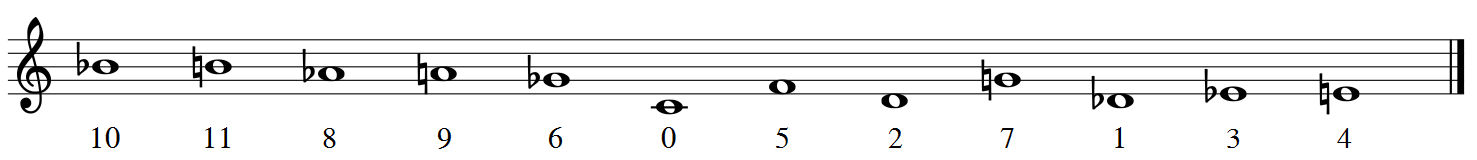
\includegraphics[width=\textwidth]{5.png}
	\bigskip\bigskip
	$$\text{IRT}^6=\left(\begin{matrix}0&1&2&3&4&5&6&7&8&9&10&11\\4&5&2&3&0&6&11&8&1&7&9&10\\\end{matrix}\right)$$
	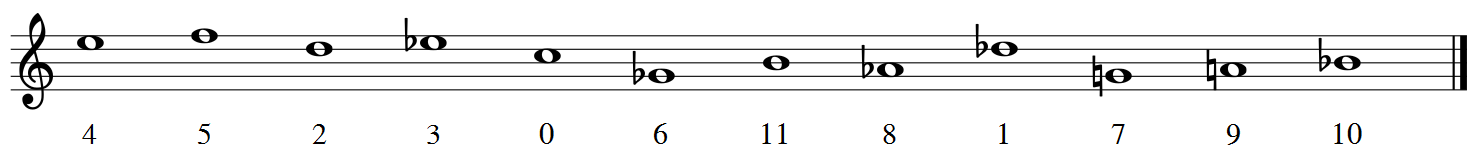
\includegraphics[width=\textwidth]{8.png}
		
		Estas series tienen muchos elementos en com\'un: todas comienzan o acaban por Mi$\natural$ o por Si$\flat$, lo que permite enlazar unas series con otras por medio del un\'isono o del tritono; se mantienen los intervalos de tritono en sus lugares originales o retr\'ogrados, y coinciden en las dos primeras y las dos \'ultimas notas dos a dos.
		
		Se han realizado estudios -- como el de Martha Hyde \cite{hyde} -- en los que se limitan las series utilizadas en la Suite a cuatro: T$^0$, T$^6$, I e IT$^6$, pero ya que el objetivo de este texto no es analizar la obra entera se dejar\'a esta cuesti\'on para an\'alisis posteriores.
		
	\subsection{Descripci\'on de la Suite op. 25}
		Schoenberg realiza en la serie $\sigma$ una partici\'on triple; es decir, la serie se divide en tres tetracordios, y cada uno de ellos contiene un intervalo de tritono. El \'ultimo tetracordio, si se retrograda, consta de las notas 10 -- 9 -- 0 -- 11, que en notaci\'on germ\'anica es la secuencia BACH. Esto puede ser un homenaje al compositor Johann Sebastian Bach (1685--1750), ya que Schoenberg admiraba a los grandes compositores anteriores a \'el por las estructuras formales de sus obras. \cite{xiao}
		
		Otro posible homenaje a Bach y sus contempor\'aneos barrocos es precisamente la forma de la obra: es una Suite, g\'enero cultivado durante los siglos XVII y XVIII que se compone de una variedad de danzas. La Suite de Schoenberg est\'a formada por seis danzas: un Preludio, una Gavota, una Musette, un Intermezzo -- que no tiene influencia barroca sino m\'as bien de Brahms, otro modelo para Schoenberg --, un Minueto con Tr\'io y una Giga. Adem\'as, el estilo, la textura -- contrapunt\'istica, t\'ipicamente barroca -- y la estructura de cada danza se corresponden con los estilos, texturas y estructuras de las danzas hom\'onimas del periodo bachiano.
        
        Por ser \'esta su primera obra totalmente dodecaf\'onica, Schoenberg la utiliz\'o como una muestra al mundo de las posibilidades de su nuevo m\'etodo compositivo. Fue tambi\'en por lo que tom\'o un formato tan variado como una Suite: as\'i pod\'ia en una misma obra componer con estilos tan distintos como los de las distintas danzas.
        
        Al componer la obra, Schoenberg trata cada tetracordio como una subunidad individual. Los superpone contra otras series del espectro tambi\'en divididas, o utiliza sus notas como un solo acorde cuatr\'iada. Estas divisiones no s\'olo sirven para hacer la serie m\'as reconocible o a\~nadir cohesi\'on a la obra, sino que adem\'as facilitan el desarrollo de la serie espec\'ificamente en el estilo de cada danza.
		
	\subsection{An\'alisis de la Musette}
	\label{musette}
		En el tercer movimiento de la Suite, la Musette, Schoenberg recrea la danza barroca que toma su nombre del instrumento hom\'onimo: la \emph{cornamusa}, de la familia de la gaita. La m\'usica compuesta para estos instrumentos suele consistir en una melod\'ia acompa\~nada por una nota pedal, que se traduce aqu\'i en la presencia de un bord\'on sobre el Sol$\natural$ (nota 7). Esta nota se extrae de cada una de las series utilizadas y se forma con ella un ostinato r\'itmico en la mano izquierda del piano. Con el resto de sonidos de cada serie, Schoenberg vuelve a emular el estilo de la danza barroca y articula un discurso polif\'onico a dos voces con ritmos esencialmente cortos.
		
		A partir de la doble barra del comp\'as 9, el Re$\flat$ (nota 1) acompa\~na a Sol$\natural$ y ambos crean un doble bord\'on en la mano izquierda. La elecci\'on de esas dos notas est\'a estrechamente relacionada con la tradicional relaci\'on de quinta justa formada por Sol$\natural$ y Re$\natural$ en la m\'usica tonal. Schoenberg sustituye las quintas justas tonales por los tritonos dodecaf\'onicos, subrayando a\'un m\'as su <<emancipaci\'on de la disonancia>>.
		
		Adem\'as de las similitudes texturales, r\'itmicas y arm\'onicas, la Musette de Schoenberg comparte estructura formal con las danzas barrocas. Y esta semejanza es quiz\'as la m\'as notable, ya que fue la b\'usqueda de estructura formal lo que inspir\'o a Schoenberg a desarrollar su m\'etodo compositivo. La Musette barroca, como todos los movimientos de danza, presenta una estructura binaria con simetr\'ia tonal: empieza y acaba por la misma tonalidad, mientras que el centro es zona de desarrollo. Schoenberg despoja de funcionalidad tonal a esa simetr\'ia, madre de la forma sonata, y la aplica a su composici\'on dodecaf\'onica.
		
		En este movimiento se pueden diferenciar a simple vista tres secciones, divididas en los compases 9 y 20, debido a cambios de textura, figuraci\'on y tempo. En la segunda secci\'on se le a\~nade melod\'ia a la mano izquierda del piano, dejando m\'as camuflado el bord\'on que en la primera secci\'on, adem\'as de que \'este se vuelve doble, mientras que vuelve a aparecer claramente en la tercera secci\'on. Tambi\'en en la segunda secci\'on aparece una nueva figuraci\'on, que es la semicorchea; y, por \'ultimo, en los dos compases de divisi\'on aparecen dos \emph{a tempo}, que marcan el final de las dos primeras secciones tras dos zonas de variabilidad r\'itmica. \cite{clercq}
		
		Para que esta estructura tr\'iptica sea una forma binaria, la primera y la \'ultima parte deben mantener un parecido, que se observa a trav\'es del an\'alisis de las series utilizadas en el movimiento. Estas series son T$^0$, T$^6$, I e IT$^6$.
		
		En la Musette, Schoenberg hace un uso casi absoluto de la tripartici\'on serial, hasta el punto de individualizar los tetracordios por separado y concederles privilegios seriales, como la retrogradaci\'on. Por ejemplo, en el comp\'as 7, en la voz inferior de la mano derecha aparece el tetracordio 4 -- 5 -- 2 -- 3, que es o bien el primer tetracordio de RIT$^6$ o la retrogradaci\'on del tercer tetracordio de IT$^6$, mientras que los otros dos tetracordios de IT$^6$, 10 -- 9 -- 7\footnote{La nota 7 aparece como bord\'on y no en la misma voz que el resto del tetracordio, por lo que su posici\'on es tambi\'en excepcional.} -- 1 en la voz superior y 8 -- 11 -- 6 -- 0 en la mano izquierda, aparecen en el orden correcto. Entonces no se puede analizar el comp\'as como RIT$^6$, sino indicar que hay una alteraci\'on puntual de IT$^6$.
		
		Por tanto, es muy complicado analizar esta obra en su totalidad, ya que la flexibilidad en la ordenaci\'on de los tetracordios puede generar situaciones muy ambiguas. Debido a estas fragmentaciones y a las variadas combinaciones de tetracordios originales y retr\'ogrados, se escucha un \'area de desarrollo hacia la secci\'on media del movimiento. En cambio, las series al principio y al final de la pieza se presentan casi \'integramente, como una exposici\'on y reexposici\'on. He aqu\'i un v\'inculo con la simetr\'ia de las formas binarias tonales. \cite{clercq}
		
		Es m\'as, incluso el orden de las series utilizadas en la primera y en la \'ultima secci\'on coinciden, exceptuando dos repeticiones consecutivas y las series T$^0$ finales, que act\'uan como una cadencia serial:
		
		\[\begin{array}{*{12}c}
			\mathbf{c}.\mathbf{1}&\text{T}^0&\text{IT}^6&\text{T}^6&\text{I}&\text{T}^0&\text{I}&\text{T}^6&
				\begin{matrix}\text{IT}^6&\text{IT}^6\\
				\end{matrix}
			&&&\mathbf{c}.\mathbf{9}\\
			\mathbf{c}.\mathbf{22}&\text{T}^0&\text{IT}^6&\text{T}^6&\text{I}&\text{T}^0&
				\begin{matrix}
				\text{I}&\text{I}\\
				\end{matrix}
			&\text{T}^6&\text{IT}^6&\text{T}^0&\text{T}^0&\mathbf{c}.\mathbf{31}\\\end{array}\]
		
		%En el Anexo \ref{app:score}, p\'agina \pageref{app:score}, 
		A continuaci\'on
		se encuentra el an\'alisis serial completo de la Musette:
		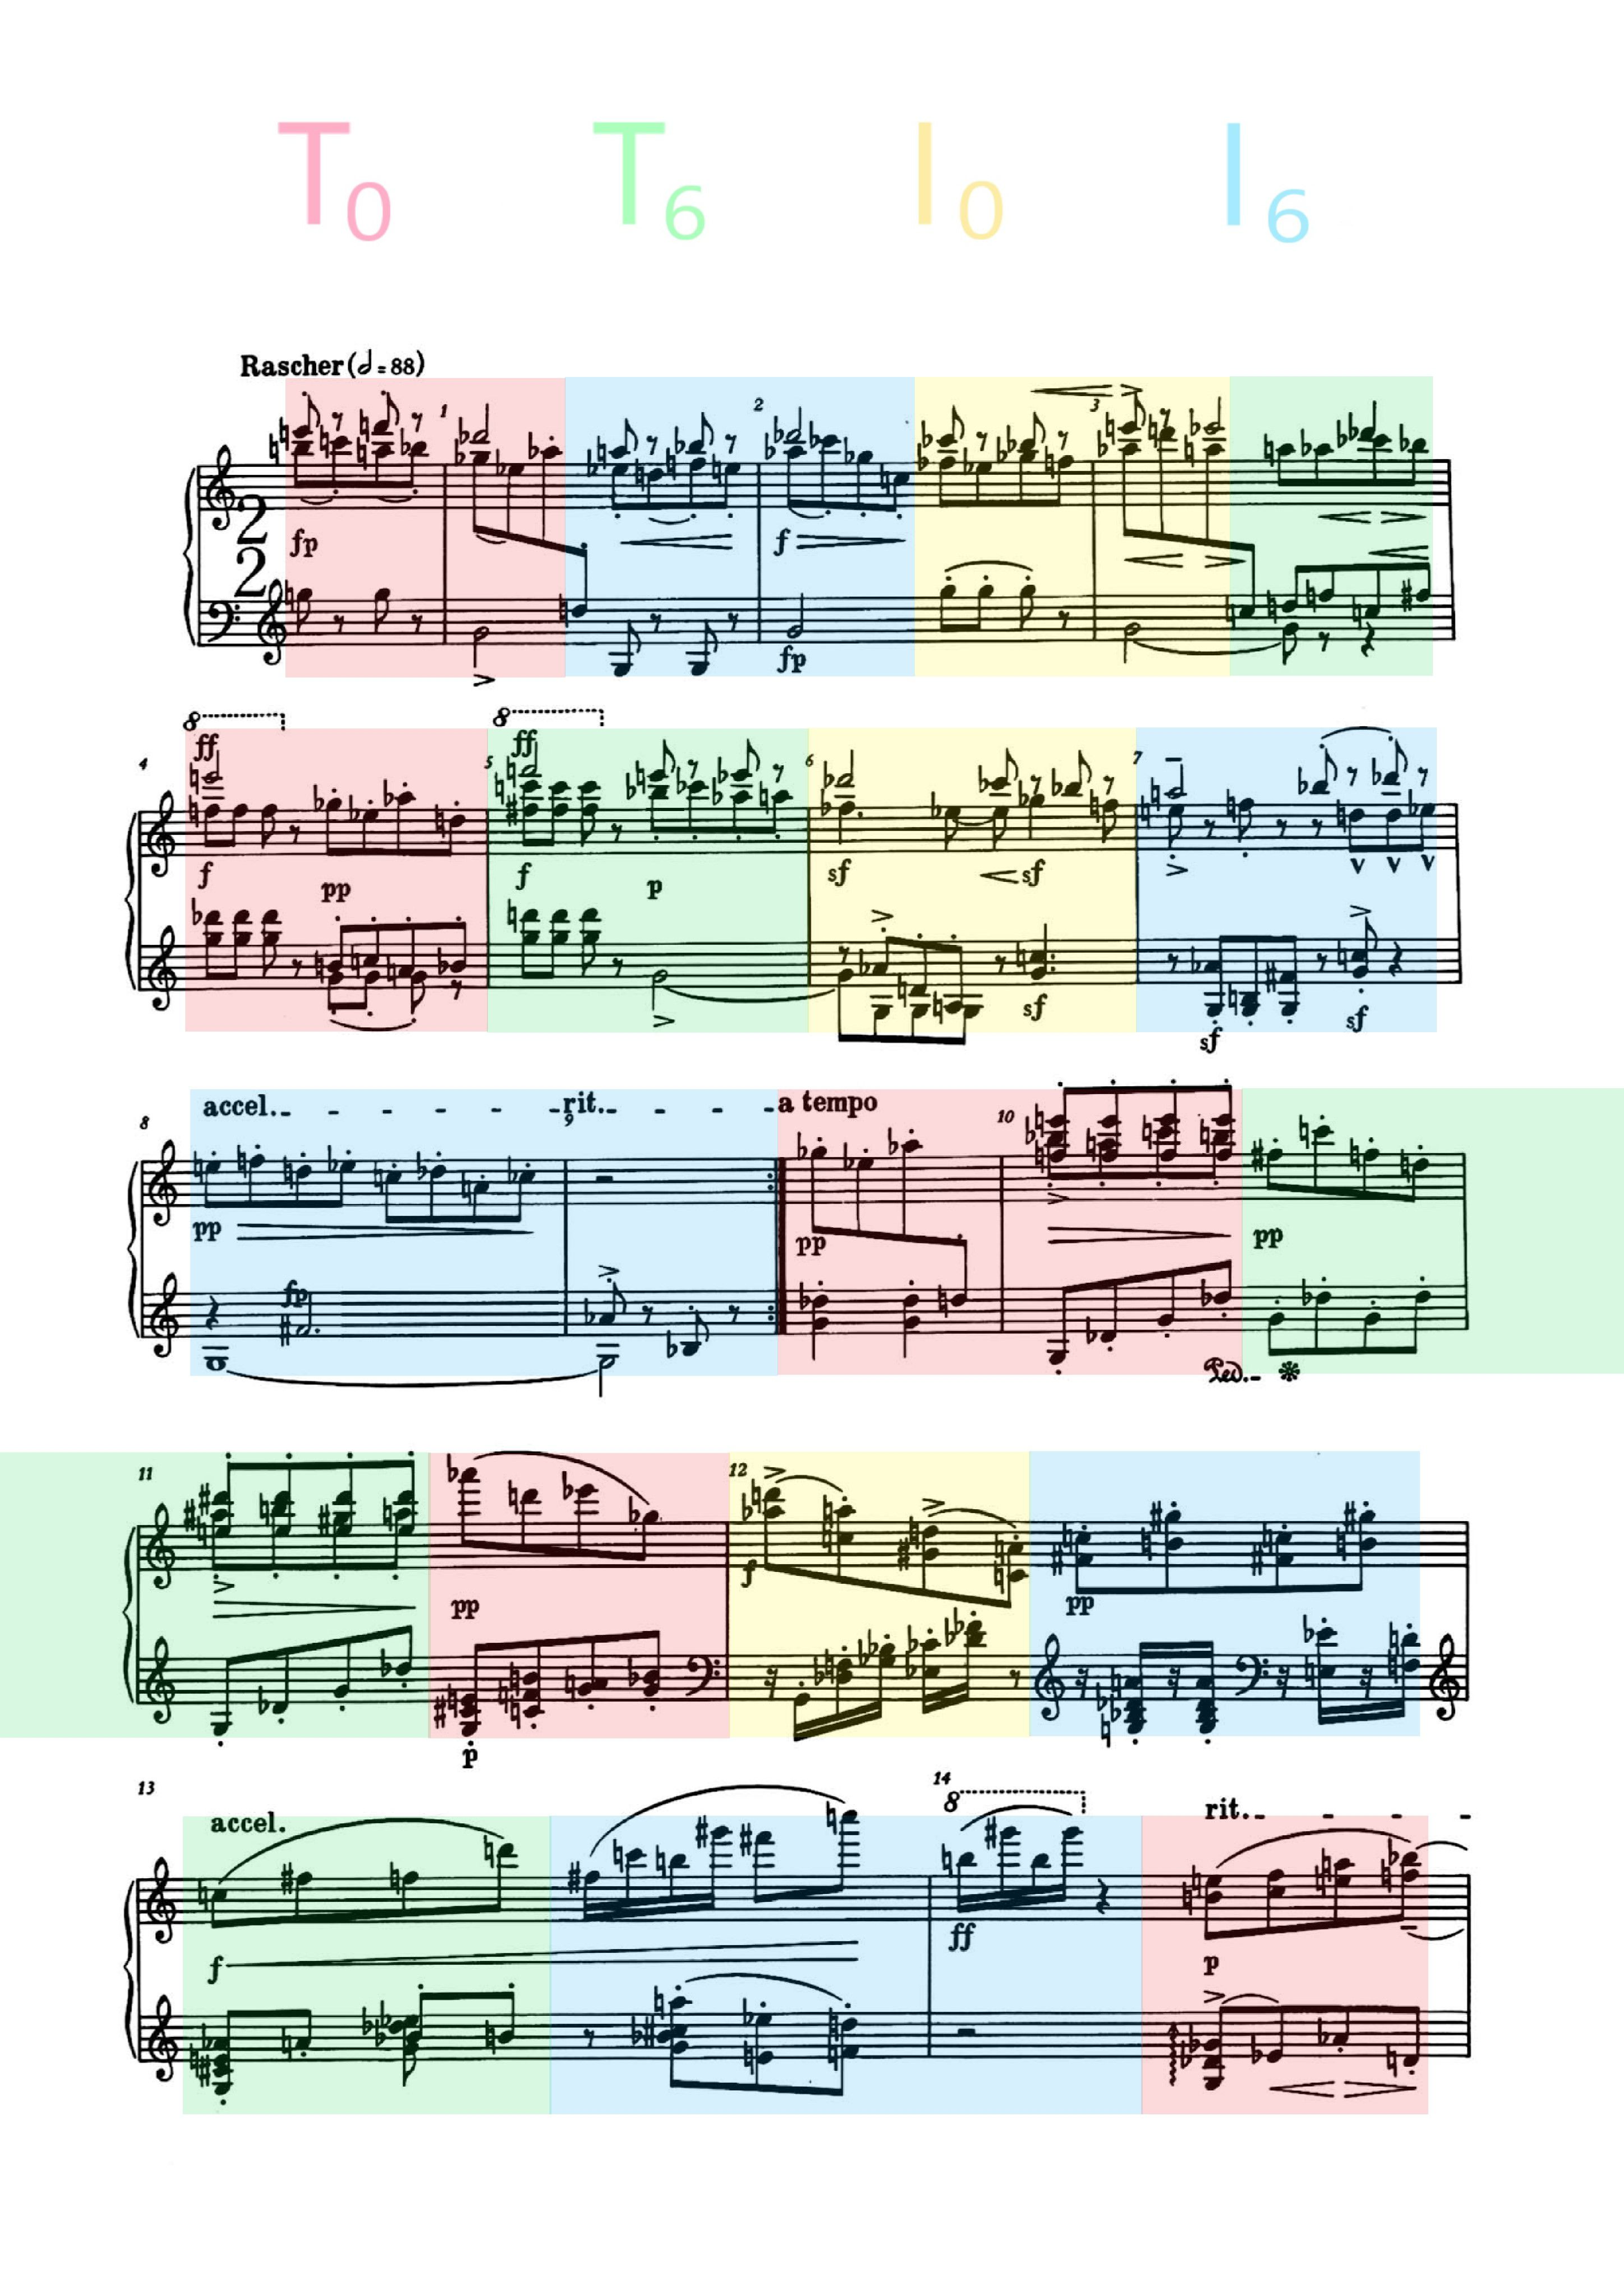
\includepdf[pages=-]{Anexos/Musette.pdf}